\documentclass[a4paper, 12pt]{article}
\usepackage[top=2cm, bottom=2cm, left=2.5cm, right=2.5cm]{geometry}
\usepackage[utf8]{inputenc}
\usepackage{hyperref}
\usepackage{graphicx}
\usepackage{amsmath}


\graphicspath{{img/}}

\begin{document}
\textbf{UNIVERSIDADE TECNOLÓGICA FEDERAL DO PARANÁ}\\
\centerline{\underline{Biologia Computacional e Sistêmica | PPGBIOINFO}}\\\\
\textbf{ALUNO:} Ricardo Medeiros da Costa Junior   \textbf{RA:} a1598996 \\
\textbf{DISCIPLINA:} Reconhecimento de Padrões\\
\textbf{ATIVIDADE:} Exercício 1, 2 e 3 - Revisão Probabilidade, Teoria da Decisão Bayesiana e Classificadores Não Supervisionados \\
\begin{enumerate}
  \item Revisão de Probabilidades
\begin{itemize} 
\item Sobre as características, defina intervalos de valores para cada uma delas de forma que as separem em 'pequena', 'media' e 'grande'.
  \begin{description}
  \item[omprimento Sépala ] [4.3,7.9]
    \begin{itemize}
    \item Pequena {[}4.3,5.5{]}
    \item Média {[}5.6,6.7{]}
    \item Grande {[}6.8,7.9{]}      
    \end{itemize}
  \end{description}
  \begin{description}
  \item[Largura Sépala ] [2,4.4]
    \begin{itemize}
    \item Pequena {[}2,2.8{]}
    \item Média {[}2.9,3.6{]}
    \item Grande {[}3.7,4.4{]}      
    \end{itemize}
  \end{description}
  \begin{description}
  \item[Comprimento Pétala ] [1,6.9]
    \begin{itemize}
    \item Pequena {[}1,2.96{]}
    \item Média {[}2.97,4.92{]}
    \item Grande {[}4.93,6.9{]}      
    \end{itemize}
  \end{description}
  \begin{description}
  \item[Largura Pétala ] [0.1,2.5]
    \begin{itemize}
    \item Pequena {[}0.1,0.9{]}
    \item Média {[}1,1.7{]}
    \item Grande {[}1.8,2.5{]}      
    \end{itemize}
  \end{description}

\item Após a definição dos intervalos, construa a matriz de distribuição de frequências e, a partir dessa matriz defina os seguintes itens:\\
  \begin{figure}[ht!]
    \centering
    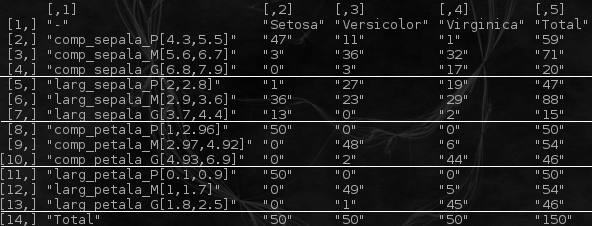
\includegraphics[width=150mm]{img1.png}
    \caption{Matriz de Distribuição}
  \end{figure}

\item Formalize o espaço amostral;\\\\
  Como cada flor pode ser Iris-setosa, Iris-versicolor e Iris-virginica, então o espaço amostral $\Omega = \{\omega_1, \omega_2, \omega_3\} \Rightarrow  \Omega = \{$ Iris-setosa, Iris-versicolor, Iris-virginica $\} $
  Por definição, é considerado o espaço todo $\Omega$ e o conjunto vazio $\emptyset$ como eventos. O primeiro é denomidado \emph{evento certo} e o segundo, \emph{evento impossível}:\\
  $$P(\Omega)=1, P(\emptyset)=0$$
  Partindo dessa perspectiva, como são 150 amostras, ou seja há 150 pontos amostrais. Então a cardinalidade do espaço amostral: $\left\vert{\Omega}\right\vert = 150$ temos $P(\Omega)=1 \Rightarrow P(\Omega)=150/150$

\item A probabilidade de cada resultado possível (probabilidades a \emph{priori});\\\\
  Seja A um evento qualquer, a probabilidade a \emph{priori} deste acontecer é dado por $$P(A)=\frac{\left\vert{A}\right\vert}{\left\vert{\Omega}\right\vert}$$\\
  onde $\left\vert{A}\right\vert$ é a cardinalidade de A e $\left\vert{\Omega}\right\vert$ a cardinalidade de $\Omega$\\\\
  \textbf{Legenda Eventos}\\
  \begin{itemize}
    \item S = Setosa
    $$P(S)=\frac{50}{150} \Rightarrow P(S)=\frac{1}{3} \Rightarrow \boxed{P(S)\approx33\%}$$
    \item Ve = Versicolor
    $$P(Ve)=\frac{50}{150} \Rightarrow P(Ve)=\frac{1}{3} \Rightarrow \boxed{P(Ve)\approx33\%}$$
    \item Vi = Virginica
    $$P(Vi)=\frac{50}{150} \Rightarrow P(Vi)=\frac{1}{3} \Rightarrow \boxed{P(Vi)\approx33\%}$$     \item CSP = Comprimento Sépala Pequena
    $$P(CSP)=\frac{59}{150} \Rightarrow \boxed{P(CSP)\approx39\%}$$      
    \item CSM = Comprimento Sépala Média
    $$P(CSM)=\frac{71}{150} \Rightarrow \boxed{P(CSM)\approx47\%}$$      
    \item CSG = Comprimento Sépala Grande
    $$P(CSG)=\frac{20}{150} \Rightarrow P(CSG)=\frac{2}{15} \Rightarrow \boxed{P(CSG)\approx13\%}$$      
    \item LSP = Largura Sépala Pequena
    $$P(LSP)=\frac{47}{150} \Rightarrow \boxed{P(LSP)\approx31\%}$$      
    \item LSM = Largura Sépala Média
    $$P(LSM)=\frac{88}{150} \Rightarrow \boxed{P(LSM)\approx58\%}$$      
    \item LSG = Largura Sépala Grande
    $$P(LSG)=\frac{15}{150} \Rightarrow P(LSG)=\frac{1}{10} \Rightarrow \boxed{P(LSG)=10\%}$$      
    \item CPP = Comprimento Pétala Pequena
    $$P(CPP)=\frac{50}{150} \Rightarrow P(CPP)=\frac{1}{3} \Rightarrow \boxed{P(CPP)\approx33\%}$$      
    \item CPM = Comprimento Pétala Média
    $$P(CPM)=\frac{54}{150} \Rightarrow P(CPM)=\frac{9}{25} \Rightarrow \boxed{P(CPM)\approx36\%}$$      
    \item CPG = Comprimento Pétala Grande
    $$P(CPG)=\frac{46}{150} \Rightarrow \boxed{P(CPG)\approx30\%}$$      
    \item LPP = Largura Pétala Pequena
    $$P(LPP)=\frac{50}{150} \Rightarrow P(LPP)=\frac{1}{3} \Rightarrow \boxed{P(LPP)\approx33\%}$$      
    \item LPM = Largura Pétala Média
    $$P(LPM)=\frac{54}{150} \Rightarrow \boxed{P(LPM)\approx36\%}$$      
    \item LPG = Largura Pétala Grande
    $$P(LPG)=\frac{46}{150} \Rightarrow \boxed{P(LPG)\approx30\%}$$      
    
  \end{itemize}
  

\item Defina pelo menos 3 eventos e calcule a probabilidade de cada um dos eventos;\\\\
  Foi realizado no exercício anterior.

\item Descrever/Comente como a escolha das características (eventos) diferentes modificaram (ou não) os resultados;\\\\
  Modificou que se caso usarmos um evento cujo possui mais pontos amostrais, a probabilidade será maior que um evento que possui menos pontos amostrais.

\item Defina pelo menos um exemplo de união de probabilidades;\\\\
  A legenda será a mesma utilizada nos exercícios anteriores.\\
  $$P(CSM \cup S) = P(CSM) + P(S) - P(CSM \cap S) \Rightarrow$$
  $$P(CSM \cup S) = \frac{71}{150} + \frac{1}{3} - \frac{1}{50} \Rightarrow$$
  $$P(CSM \cup S) = \frac{71+50-3}{150} \Rightarrow$$
  $$P(CSM \cup S) = \frac{118}{150} \Rightarrow$$    
  $$\boxed{P(CSM \cup S) \approx 78\%} $$


\item Defina pelo menos um exemplo de interseção de probabilidades;\\
  $$P(LPG \cap Vi) = 45 $$

\item Defina pelo menos 3 exemplos de probabilidades condicionais. \\\\
  Para dois eventos quaisquer A e B, sendo $P(B)>0$, definimos a \emph{probabilidade condicional de} A \emph{dado} B, $P(A|B)$, como sendo:\\
  $$P(A|B)=\frac{P(A \cap B)}{P(B)}$$\\
  Utilizando a legenda dos exercícios anteriores:\\
  \begin{enumerate}
  \item $P(LSP|Ve)=\frac{P(LSP \cap Ve)}{P(Ve)} \Rightarrow$
    $$P(LSP|Ve)=\frac{\frac{23}{150}}{\frac{1}{3}} \Rightarrow$$
    $$P(LSP|Ve)=\frac{23}{150}\cdot3 \Rightarrow$$
    $$P(LSP|Ve)=\frac{23}{50} \Rightarrow$$
    $$\boxed{P(LSP|Ve)\approx46\%} $$
    
  \item $P(CPP|S)=\frac{P(CPP \cap S)}{P(S)}$
   $$P(CPP|S)=\frac{\frac{1}{3}}{\frac{1}{3}} \Rightarrow$$
   $$P(CPP|S)=\frac{1}{3}\cdot3 \Rightarrow$$
   $$P(CPP|S)=1 \Rightarrow$$
   $$\boxed{P(CPP|S)=100\%} $$
     
  \item $P(LPM|Vi)=\frac{P(LPM \cap Vi)}{P(Vi)}$
   $$P(LPM|Vi)=\frac{\frac{1}{30}}{\frac{1}{3}} \Rightarrow$$
   $$P(LPM|Vi)=\frac{1}{30}\cdot3 \Rightarrow$$
   $$P(LPM|Vi)=\frac{1}{10} \Rightarrow$$
   $$\boxed{P(LPM|Vi)=10\%} $$
     
  \end{enumerate}
  

\end{itemize}
\item Teoria de Decisão Bayesiana
  \begin{itemize}
  \item Sobre as características, use as amostras nas definições originais e crie partições para a construção das curvas de FDP e Probabilidade a Posteriori.\\\\
    Para criar as partições para construção da curva FDP foi utilizado a desigualdade $k\Delta i \ge max-min$ para achar o valor de $k$ que irá dividir as partições. Para determinar o valor de $k$ foi aplicado a fórmula de \textbf{Sturges}, no qual $k$ é o menor inteiro $k>1+3,32\log(n)$.\\
    \begin{description}
    \item[Valor de $k$]
      $$k>1+3,32\log(n) \Rightarrow$$
      $$k>1+3,32\cdot2.178 \Rightarrow$$
      $$k>1+7,224 \Rightarrow $$
      $$k>8,224 \Rightarrow $$
      $$\boxed{k=9} $$
    \item[Comprimento Sépala: mín 4,3; máx 7,9]
      $$9\Delta i \ge 7,9 - 4,3 \Rightarrow $$
      $$\Delta i \ge \frac{3,6}{9} \Rightarrow $$
      $$ \boxed{\Delta i \ge 0,4} $$
    \item[Largura Sépala: mín 2; máx 4,4]
      $$9\Delta i \ge 4,4 - 2 \Rightarrow $$
      $$\Delta i \ge \frac{2,4}{9} \Rightarrow $$
      $$\boxed{\Delta i \ge 0,27}$$
    \item[Comprimento Pétala: mín 1; máx 6,9]
      $$9\Delta i \ge 6,9 - 1 \Rightarrow $$
      $$\Delta i \ge \frac{5,9}{9} \Rightarrow $$
      $$\boxed{\Delta i \ge 0,66}$$
    \item[Largura Pétala: mín 0,1; máx 2,5]
      $$9\Delta i \ge 2,5 - 0,1 \Rightarrow $$
      $$\Delta i \ge \frac{2,4}{9} \Rightarrow $$
      $$\boxed{\Delta i \ge 0,27}$$
    \end{description} \\
    Após isso foi realizado a contagem de cada característica em cada intervalo. Nota-se pelas tabelas que os intervalos são fechados pela esquerda e aberto pela direita. Isso foi adotado para todas as tabelas.\\
  \begin{figure}[h!]
    \centering
    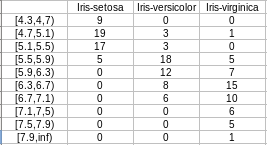
\includegraphics[width=80mm]{img2.png}
    \caption{Comprimento Sépala}
  \end{figure}
  \begin{figure}[h!]  
    \centering
    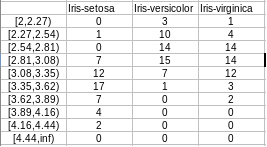
\includegraphics[width=80mm]{img3.png}
    \caption{Largura Sépala}
  \end{figure}
  \begin{figure}[h!]  
    \centering    
    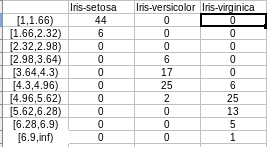
\includegraphics[width=80mm]{img4.png}
    \caption{Comprimento Pétala}
  \end{figure}
  \begin{figure}[h!]  
    \centering
    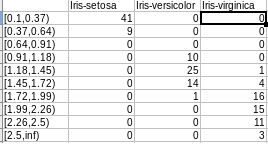
\includegraphics[width=80mm]{img5.png}
    \caption{Largura Pétala}
  \end{figure}
  \\\\
  
\item Aplicar a Função de Densidade e Probabilidade (FDP) condicional como visto em aula para as 4 características e 3 classes do conjunto de dados, gerando os 4 gráficos \\\\
    \begin{figure}[h!]
    \centering
    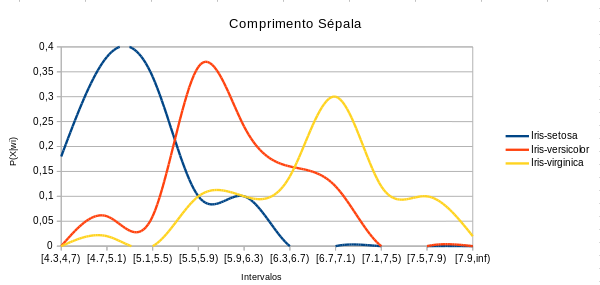
\includegraphics[width=80mm]{img6.png}
    \caption{Comprimento Sépala}
    \end{figure}

    \begin{figure}[h!]
    \centering
    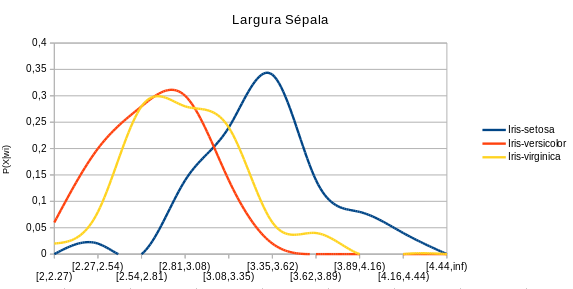
\includegraphics[width=80mm]{img7.png}
    \caption{Largura Sépala}
    \end{figure}

    \begin{figure}[h!]
    \centering
    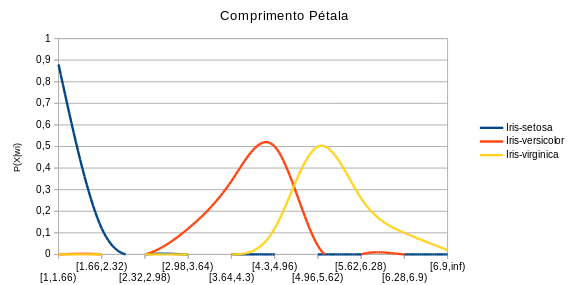
\includegraphics[width=80mm]{img8.png}
    \caption{Largura Pétala}
    \end{figure}

    \begin{figure}[h!]
    \centering
    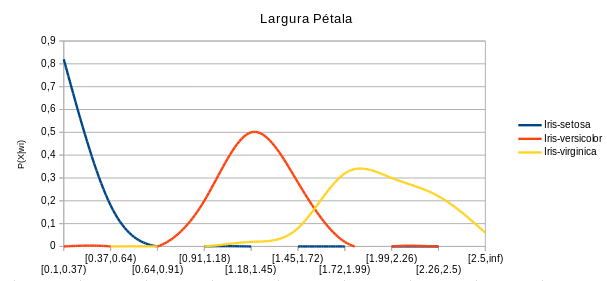
\includegraphics[width=80mm]{img9.png}
    \caption{Largura Pétala}
    \end{figure}

  \item Aplicar a regra de decisão Bayesiana (probabilidade a posteriori) como visto em aula para as 4 características e 3 classes do conjunto de dados, gerando os 4 gráficos. (Nota-se que em alguns as probabilidades passaram de 1\% por causa da suavização da planilha eletrônica)\\\\\\\\
    \begin{figure}[h!]
    \centering
    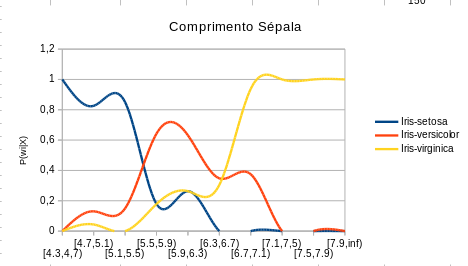
\includegraphics[width=80mm]{img10.png}
    \caption{Comprimento Sépala}
    \end{figure}

    \begin{figure}[h!]
    \centering
    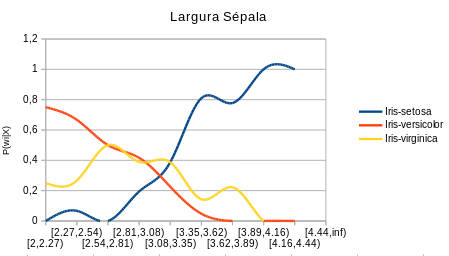
\includegraphics[width=80mm]{img11.png}
    \caption{Largura Sépala}
    \end{figure}

    \begin{figure}[h!]
    \centering
    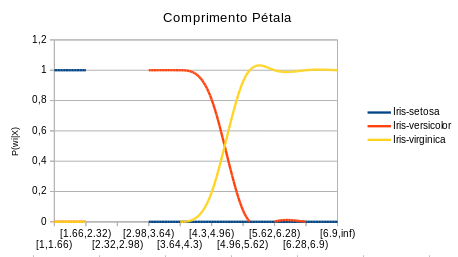
\includegraphics[width=80mm]{img12.png}
    \caption{Largura Pétala}
    \end{figure}

    \begin{figure}[h!]
    \centering
    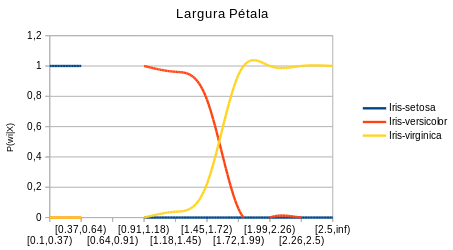
\includegraphics[width=80mm]{img13.png}
    \caption{Largura Pétala}
    \end{figure}
    

  \item Descrever como a escolha das características (eventos) diferentes modificaram (ou não) os resultado\\\\
    Nota-se, observando os gráficos e analisando as probabilidades, que é possível determinar facilmente qual classe é por meio de algumas característica. Ou seja, há características em que as flores são bem diferentes, dessa forma torna-se aconselhável utilizar essas características ao criar o modelo.
    
  \end{itemize}
\item Classificadores Não Supervisionados
  \begin{itemize}
    \item Ligação média e Distância Euclidiana;
    \begin{figure}[h!]
    \centering
    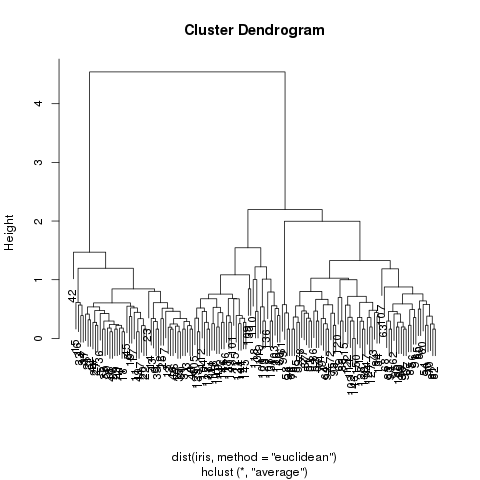
\includegraphics[width=80mm]{img14.png}
    \end{figure}
    
    \item Ligação média e Correlação de Pearson;
    \begin{figure}[h!]
    \centering
    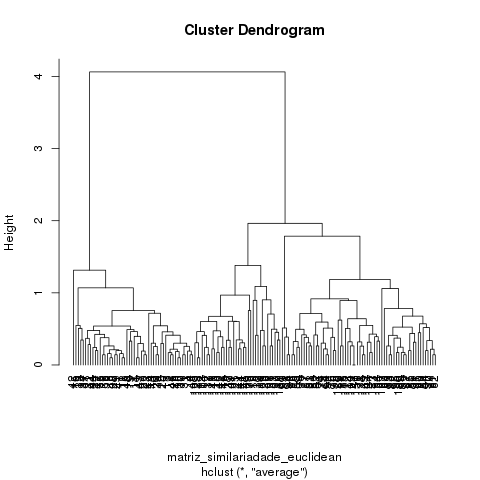
\includegraphics[width=80mm]{img15.png}
    \end{figure}

  \end{itemize}

\end{enumerate}
\end{document}
